\documentclass[10pt,conference,compsocconf]{IEEEtran}

\usepackage{hyperref}
\usepackage{graphicx}
\usepackage{amsmath}
\usepackage{booktabs}
\usepackage[font=small,skip=3pt]{caption}
\usepackage{microtype}
\setlength{\textfloatsep}{9pt plus 2pt minus 2pt}

\newcommand{\hare}{\texttt{HAREHAB1}}

\begin{document}
\title{Predicting Heart Disease from Survey Answers}

\author{
  Clémentine BAUDOU, Lucas OLIVIER\\
  \textit{Team ML-Formula1-Team --- CS-433 Machine Learning, EPFL, Switzerland}
}

\maketitle

\begin{abstract}
We predict coronary heart disease, heart attack or angina (MICHD) from the 321 answers of BRFSS 2015 survey respondents with NumPy only, combining a codebook-based preprocessing, gradient-boosted trees implemented from scratch and neural networks.
Our main finding concerns the data: questions answered by fewer than 1\% of respondents, discarded by a missing-value filter, carry strong information through the survey's skip logic.
The final model reaches a cross-validated F1 of 0.448 (0.415 for logistic regression on raw features) and a test F1 of 0.459, first place at submission time; an ablation and a leakage check quantify each step.
\end{abstract}

\begin{figure*}[t]
  \centering
  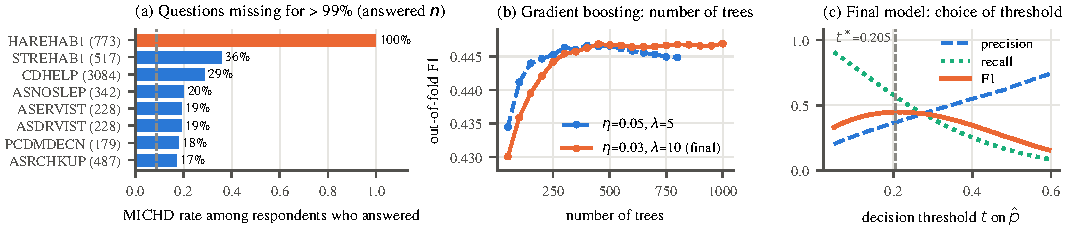
\includegraphics[width=\textwidth]{figures/report_overview}
  \vspace{-6mm}
  \caption{(a) MICHD rate among respondents who answered the 8 most informative questions missing for more than 99\% of respondents (dashed: overall rate, 8.8\%). (b) Out-of-fold F1 of the GBDT as trees are added, for two regularization settings. (c) Out-of-fold precision, recall and F1 of the final model versus the decision threshold.}
  \label{fig:overview}
  \vspace{-4mm}
\end{figure*}

\section{Introduction}
The Behavioral Risk Factor Surveillance System (BRFSS) is a US telephone survey on health behaviours and chronic conditions~\cite{brfss2015}.
We get $N=328{,}135$ labelled and $109{,}379$ test respondents with $D=321$ raw answers each (147 columns are more than half empty).
Only 8.8\% are positive, so predicting ``healthy'' for everybody is 91.2\% accurate but useless; submissions are ranked by the F1 score $2\,\mathrm{TP}/(2\,\mathrm{TP}+\mathrm{FP}+\mathrm{FN})$.
Everything is written in NumPy. We contribute a survey-aware preprocessing (Sec.~\ref{sec:prep}), a NumPy gradient boosting (Sec.~\ref{sec:gbdt}) and an ablation with a leakage check (Sec.~\ref{sec:results}).

\section{Models and Methods}

\subsection{Evaluation protocol}
\label{sec:protocol}
All results use the same 5-fold cross-validation (CV, seed 42); every preprocessing statistic (kept columns and levels, medians, means, bin edges) is fitted on the training folds only.
A model outputs a probability $\hat p$ and predicts MICHD if $\hat p\ge t$.
With rare positives $t=0.5$ is far from optimal; for calibrated probabilities the F1-optimal threshold is half the best F1~\cite{lipton2014} ($\approx$0.22 here).
We report the mean $\pm$ std over folds of the F1 at each fold's best threshold, and the \emph{out-of-fold} (OOF) F1 of the pooled held-out probabilities at one global threshold $t^\ast$, which mimics the submission.

\subsection{Preprocessing}
\label{sec:prep}
A first Jupyter notebook showed mostly categorical, often missing answers, hence one-hot encoding and boosted trees (\texttt{project\_overview.ipynb}).
For linear models and networks we build a one-hot design matrix.
(1) We drop 36 columns: dates, identifiers, sampling weights, phone screening, and raw answers that the codebook~\cite{brfss2015} also provides cleaned (e.g.\ \texttt{WEIGHT2}$\to$\texttt{WTKG3}).
(2) In the 65 numeric columns, 77/99 (``don't know''/``refused'') become missing, 88 (``none'') becomes 0, codes $1xx$/$2xx$ ($xx$ times per week/month) become times per month, 36 skewed counts are log-transformed, and missing values get the median plus an indicator.
(3) Columns with at most 60 distinct values are one-hot encoded (levels seen $\ge100$ times), keeping ``missing'', ``don't know'' and ``refused'' as levels, since not answering is informative.
(4) We add age$\times$sex, age$\times$general-health and squared terms, standardize and add a bias ($\approx$1{,}100 columns).

\emph{Rare optional-module questions.} The first pipeline also dropped the 30 columns missing for more than 99\% of respondents.
They come from optional state modules and follow-up (skip) questions, and their answers are far from the 8.8\% base rate (Fig.~\ref{fig:overview}a).
In particular, \hare{} (``Following your heart attack, did you go to any kind of outpatient rehabilitation?'') is only asked after a reported heart attack: all 773 training respondents who answered it have MICHD (238 test respondents answered it), yet our previous model flagged only 62\% of them.
We now keep every column, and (5) add three counts: chronic conditions answered ``yes'' (11 questions), activity limitations (7), and unanswered questions ($\approx$1{,}200 columns).

\subsection{Required methods}
We implemented the six methods of Table~\ref{tab:methods} with labels $y\in\{0,1\}$, thresholding the score $\mathbf{x}^\top\mathbf{w}$ of the regressions like a probability:
gradient descent (GD) on the MSE with step $1/L$, $L$ being the largest eigenvalue of $X^\top X/N$ (power iteration; $\gamma=0.1$ diverges), 300 steps;
SGD with batch size 1, $\gamma=10^{-4}$, $3N$ steps; least squares (LS) and ridge ($\lambda=10^{-5}$) by the normal equations; logistic regression (LR) and its regularized version (Reg-LR, $\lambda=10^{-6}$) by GD with $\gamma=0.5$, 300 steps.
CV of the logistic penalty over $\lambda\in\{10^{-6},\dots,10^{-1}\}$ gives the same F1 for $\lambda\le10^{-3}$ and less above (0.411 at $10^{-1}$): with $N\gg D$ overfitting is mild. We also tried class weights and a Newton solver~\cite{esl}.

\subsection{Gradient-boosted decision trees (GBDT)}
\label{sec:gbdt}
The score $F(\mathbf{x})=F_0+\sum_{m=1}^{M}f_m(\mathbf{x})$, $\hat p=\sigma(F)$, is a sum of regression trees added greedily~\cite{friedman2001}.
Each tree minimizes a second-order expansion of the logistic loss~\cite{xgboost}: with $g_i=\hat p_i-y_i$, $h_i=\hat p_i(1-\hat p_i)$ and their sums $G,H$ over a node, a leaf gets the value $-\eta\,G/(H+\lambda)$ and a node is split where $G_L^2/(H_L+\lambda)+G_R^2/(H_R+\lambda)-G^2/(H+\lambda)$ is largest.
As in LightGBM~\cite{lightgbm}, each feature is cut once into $\le64$ bins (one per answer code, quantiles for continuous values); per-bin sums of $g$ and $h$ are obtained with \texttt{np.bincount} and all thresholds are scored at once by cumulative sums; only the smaller child's histogram is computed, the other being parent minus smaller.
Missing values form their own bin and go to the side with the larger gain, so trees need no imputation, encoding or scaling; they use the 285 raw columns and the 3 counts.
We use $M=1000$ trees of depth $\le6$, $\eta=0.03$, $\lambda=10$, a hessian sum $\ge10$ per child, and 70\% of the rows and 40\% of the features per tree.
A less regularized setting ($\eta=0.05$, $\lambda=5$) overfits after 450 trees (Fig.~\ref{fig:overview}b).

\subsection{Neural networks, ensemble and decision rule}
Each network has 128 ReLU hidden units, dropout 0.5~\cite{dropout}, input clipped to $[-10,10]$, and is trained on the logistic loss with weight decay $10^{-4}$ by Adam~\cite{adam} (batch 1024, 6 epochs, learning rate $10^{-3}$ with cosine decay~\cite{sgdr}); we average 5 networks (NN, seeds 0--4).
The final probability is $\sigma\big(\tfrac12\mathrm{logit}\,\hat p_{\mathrm{NN}}+\tfrac12\mathrm{logit}\,\hat p_{\mathrm{GBDT}}\big)$: in a grid search on the OOF probabilities every network weight in $[0.3,0.65]$ gave the same F1 ($\pm0.0005$), and logistic regression as a third member got weight 0.
Respondents who answered \hare{} are set to positive (``rehab rule''), and $t^\ast=0.205$ (Fig.~\ref{fig:overview}c).
\texttt{run.py} reproduces the submission exactly on a given machine (fixed seeds, 13 minutes); on another platform, float32 rounding changes 0.3\% of predictions.

\begin{table}[t]
\centering
\caption{Ablation (5-fold CV): rows 0--7 first round, 8--15 second round, L1--L3 leakage check; each row changes one thing vs.\ the row above (or named). Fold F1: mean $\pm$ std of per-fold best F1; OOF F1, Acc.: pooled predictions at $t^\ast$. Test F1: 0.448 (row 6), 0.459 (row 15).}
\label{tab:ablation}
\scriptsize
\setlength{\tabcolsep}{2.6pt}
\begin{tabular}{@{}rllccc@{}}
\toprule
\# & Configuration & Model & Fold F1 & OOF F1 & Acc. \\
\midrule
0 & Raw features, median imputation & LR & .4161\,$\pm$\,.0014 & .4155 & .869 \\
1 & + drop administrative columns & LR & .4161\,$\pm$\,.0019 & .4154 & .872 \\
2 & + decode special codes, log & LR & .4177\,$\pm$\,.0011 & .4173 & .870 \\
3 & + one-hot categorical answers & LR & .4326\,$\pm$\,.0014 & .4317 & .865 \\
4 & + age / health interactions & LR & .4323\,$\pm$\,.0016 & .4313 & .867 \\
5 & + class weights (positives $\times$3) & LR & .4322\,$\pm$\,.0016 & .4312 & .867 \\
6 & 5 networks (previous submission) & NN & .4343\,$\pm$\,.0021 & .4339 & .880 \\
7 & Blend of rows 4 and 6 & LR+NN & .4335\,$\pm$\,.0016 & .4330 & .874 \\
\midrule
8 & Row 4 + rare module questions & LR & .4406\,$\pm$\,.0014 & .4395 & .875 \\
9 & + count features & LR & .4406\,$\pm$\,.0012 & .4395 & .875 \\
10 & + Newton solver, $\lambda{=}10^{-4}$ & LR & .4399\,$\pm$\,.0009 & .4390 & .877 \\
11 & 5 networks, new features & NN & .4420\,$\pm$\,.0016 & .4411 & .871 \\
12 & + 128 units, cosine schedule & NN & .4457\,$\pm$\,.0021 & .4451 & .881 \\
13 & Gradient-boosted trees & GBDT & .4476\,$\pm$\,.0021 & .4469 & .879 \\
14 & Average of rows 12 and 13 & NN+GBDT & .4489\,$\pm$\,.0014 & .4476 & .876 \\
15 & + rehab rule (final model) & NN+GBDT & \textbf{.4489\,$\pm$\,.0014} & \textbf{.4476} & \textbf{.876} \\
\midrule
L1 & Row 12 without \hare{} & NN & .4368\,$\pm$\,.0012 & .4366 & .878 \\
L2 & Row 13 without \hare{} & GBDT & .4384\,$\pm$\,.0024 & .4378 & .882 \\
L3 & Average of L1 and L2 & NN+GBDT & .4399\,$\pm$\,.0018 & .4392 & .880 \\
\bottomrule
\end{tabular}
\vspace{-2mm}
\end{table}

\begin{table}[t]
\centering
\caption{Required methods: mean 5-fold CV F1 on Table~\ref{tab:ablation} row-4 features (std $\le$0.006); $^\dagger$singular $X^\top X$.}
\label{tab:methods}
\footnotesize
\setlength{\tabcolsep}{4pt}
\begin{tabular}{@{}lcccccc@{}}
\toprule
 & GD & SGD & LS & Ridge & LR & Reg-LR \\
\midrule
F1 & 0.4264 & 0.3952 & sing.$^\dagger$ & 0.4267 & 0.4322 & 0.4322 \\
\bottomrule
\end{tabular}
\vspace{-3mm}
\end{table}


\section{Results}
\label{sec:results}
In Table~\ref{tab:methods} the logistic models beat the regressions, which fit a linear score to binary labels; least squares fails on the collinear one-hot columns (ridge fixes it).
In the ablation (Table~\ref{tab:ablation}), one-hot encoding is the key first-round step (+0.014 OOF F1); class weights only move $t^\ast$ (0.19$\to$0.42).
In the second round, the rare module questions bring the largest gain (+0.008 for LR, rows 4$\to$8; +0.007 for the networks, rows 6$\to$11).
The counts do not help LR but trees use them heavily.
Wider networks add +0.004, the GBDT is the best single model, and their average has the best per-fold F1 ($0.4489\pm0.0014$).
The rehab rule changes nothing in CV (the models already flag every \hare{} respondent) but secures the 238 test cases; the test F1 is 0.459 (accuracy 0.887).
Without the \hare{} column (rows L1--L3) the ensemble still reaches 0.439: of the +0.014 gain over row~6, +0.005 comes from all other changes and +0.008 from this single question.

\section{Discussion and Summary}
\emph{Data before models.} Missingness encodes the survey's routing: one skip-logic answer is worth more F1 than all our other changes.
But \hare{} is target leakage~\cite{leakage}: legitimate here since it is in the test features, it is no risk factor and a screening tool could not use it.

\emph{Limitations.} F1 differences below 0.001 are noise (fold std 0.001--0.002); the gain agrees between CV (+0.014) and test (+0.011). Labels are self-reported.

\emph{Summary.} Survey-aware preprocessing, a NumPy GBDT and an ensemble raise F1 from 0.415 to 0.448 (CV), 0.459 (test).

\bibliographystyle{IEEEtran}
\bibliography{literature}

\end{document}
